
We turn to analyze real mixtures collected using RNA-seq measurements from postmortem human brains. We used data from brainspan \cite{brainspan} (\url{http://www.brainspan.org/} and limited analysis to donors older than 17 years, leaving 8 adult human donors. We therefore had eight samples from each brain region. Each expression profile is represented by a vector of 52376 measurements including transcripts counts for coding and non-coding sequences. 

%Collecting human brain measurements is not easy to task since the the tissues has to be extracted not long after the subject death. So while the expression in each tissue can be represented in more details with the advancement of the sequencing tools, the number of samples is still extremely limited. For example, in our dataset there only few dozen samples and each is representation by tens of thousands features.

RNA sequencing is becoming the main way to measure gene expression in tissues, replacing the older microarrays technology. RNA sequencing provides more quantitative measurement since it actually counts the number of RNA transcripts in a tissue, as opposed to the more qualitative microarrays measurements. As such, RNA-seq data is more suitable for demixing since the number of RNAs transcripts grows linearly with the proportion of correspondiong cells in the tissue.

To evaluate the quality of demixing, we compare the inferred hidden cell-type specific profiles to transcriptome profiles measured in population of cells sorted by their cell type. At the time we conducted the analysis the cell-type specific RNA-seq data were only available in mouse \cite{barres2014}. We mapped the genes in the human to their orthologs in mouse and computed the spearman correlation between the reconstructed profiles and each of the single cell profiles. Recently such cell-type-specific data was made available for human, which will allow us to perform better validations. 

We determined the strengths of region-to-region relatedness $\phi_{r,s}$ based on the brain-region-ontology described inf Figure ~(1). To verify that the human transcriptome measurements agree with this ontology, we first used an agglomerate hierarchical clustering over regions, by clustering expression profiles of these regions collected using microarray data by \cite{kang}. The resulting region hierarchy had very string agreement with the brain region ontology, consistent with previous reports that adult expression patterns reflect brain development \cite{zapala-2005}. The strengths of region-to-region attractive potentials $\lambda_{r,s}$ was determined as $\lambda \phi_{r,s}$ where $\lambda$ is a hyper parameter controlling the overall weight of edge potentials. 


Figure \ref{fig:human} shows ...


We compared our results with those of random baseline that was obtained by repeatedly selecting a set of 3 samples as the reconstructed profiles. It should be notated that even single cell experiments that are gathered from the same species in different experiment and from different region is only correlated to the other samples from the same type by 0.877. 
We notice that for most parts we are able to improve the reconstruction over the baseline. The use of the regions prior also improves the demixing over the demixing obtained using each brain region individually.


%   We find that in our reconstructed profiles the gene that are
%   For each of demixed profiles we performed enrichment analysis and found that ...



\begin{figure}[!hbt]
    \label{fig:human}
   (a) \hspace{120pt}(b) \hspace{120pt}(c) \hspace{120pt}
   \centering
     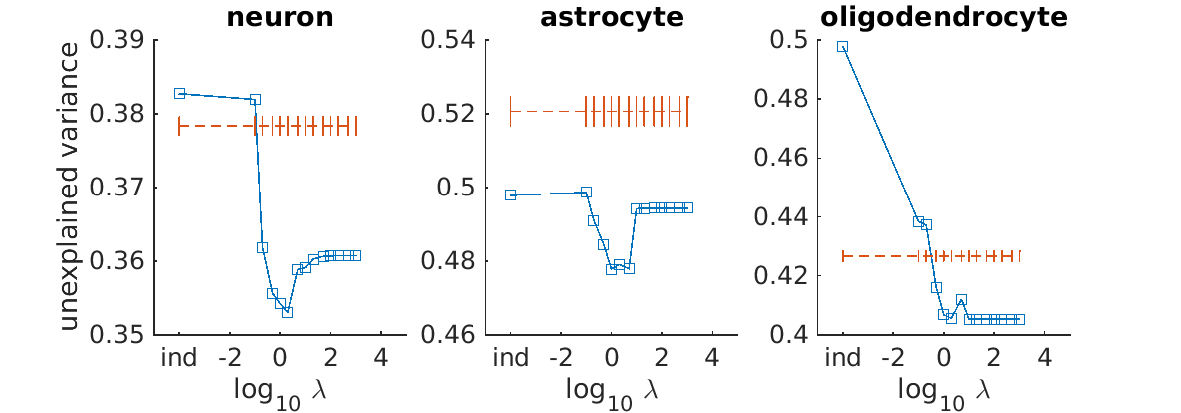
\includegraphics[width=0.99\textwidth]{3panels_var_AMY-CBC-DFC-HIP-V1C.png}
     \caption{Demixing RNA-seq data from 5 human brain regions \cite{brainspan}. Blue curve and squares correspond to the residual variance (1-\rho^2) as a function of the strength of attractive region-to-region potentials $\lambda$. Red dashed line corresponds to a best-matched-sampels baseline (see text). At the optimum, the residual unexplained variance is reduced by 7\% for neurons, 8\% for astrocytes and 5\% in oligodendrocytes.}
    
\end{figure}



[Add in the human experiment section We first verified that the brain regions in our data agree with the dev ontology: we clustered the brain regions in a hierarchical way and compared the resulting hierarchy to the dev ontology. We obtained very strong agreement …]. 
